\section{实验}

\subsection{实验设置}

\paragraph{Grounding 基准。}
我们在五个 GUI grounding 基准上评估模型的元素感知与定位能力，包括 ScreenSpot-Pro、ScreenSpot-v2、OSWorld-G、MMBench-GUI-L2 与 VisualWebBench~\citep{li2025screenspotpro, wu2024atlas, wang2025mmbench, liu2024visualwebbench_vwb}。

\paragraph{桌面与手机任务。}
OSWorld~\citep{xie2024osworld} 提供 369 个真实桌面任务，覆盖多种桌面软件；AndroidWorld~\citep{rawles2024androidworld} 提供 116 个手机任务，运行在真实 Android 模拟环境中；AndroidDaily 则补充了更贴近高频中文移动应用场景的评测。

\paragraph{通用多模态基准。}
为了验证 Step-GUI 并未因 GUI 专项训练而失去通用能力，我们还在 OCR、图表理解、数学视觉推理和一般多模态理解基准上进行测试。

\paragraph{对比方法。}
基线覆盖了当前主流基础模型与 GUI 专项模型，包括 Claude、OpenAI CUA、Gemini、UI-TARS、InternVL、MobileRL、AutoGLM、Qwen 系列与 GUI-Owl 等~\citep{claude4sonnet, claude45sonnet, openai_cua_o3, gemini2.5cu, qin2025ui_uitars1, wang2025ui_uitars2, wang2025internvl3, xu2025mobilerl, AutoGLM, glm4.6v, bai2025qwen2, ye2025mobile_mobileagentv3, Bai2025Qwen3VL}。

\subsection{主要结果}

\paragraph{GUI grounding。}
Step-GUI 在多个 grounding 基准上表现稳定且强劲。尤其是 Step-GUI-8B，在 ScreenSpot-Pro 上达到 62.6，在 OSWorld-G 上达到 70.0，在 MMBench-GUI-L2 上达到 85.6，并在 VisualWebBench 上保持非常有竞争力的表现。相比同规模或更大规模的基础模型，Step-GUI 在 GUI 元素理解和定位方面展现出显著优势。

\begin{table}[t]
\centering
\caption{多个 GUI grounding 基准上的表现。粗体为最优，带下划线为次优。}
\label{tab:gui_benchmark_performance}
\resizebox{\linewidth}{!}{
\begin{tabular}{l|ccccc}
\toprule
\textbf{模型} & ScreenSpot-Pro & ScreenSpot-v2 & OSWorld-G & MMBench-GUI-L2 & VisualWebBench \\
\midrule
OpenAI CUA & 23.4 & 87.9 & 36.4 & - & - \\
UI-TARS-1.5 & \underline{61.6} & 94.2 & - & - & - \\
SeedVL-1.5 & 60.9 & \textbf{95.2} & - & \underline{84.4} & 87.3 \\
GUI-Owl-32B & 58.0 & 93.2 & 58.0 & 83.0 & - \\
Qwen3-VL-4B-Instruct & 59.5 & 94.0 & 58.2 & - & - \\
Qwen3-VL-8B-Instruct & 54.6 & 94.4 & 58.2 & - & - \\
Qwen3-30B-A3B-Instruct & 60.5 & 94.7 & 61.0 & 79.7 & 79.7 \\
\textbf{Step-GUI-4B} & 60.0 & 93.6 & \underline{66.9} & 84.0 & \textbf{90.7} \\
\textbf{Step-GUI-8B} & \textbf{62.6} & \underline{95.1} & \textbf{70.0} & \textbf{85.6} & \underline{89.7} \\
\bottomrule
\end{tabular}}
\end{table}

\paragraph{端到端 GUI 任务。}
在 AndroidWorld 与 OSWorld 这类需要多步规划和稳定执行的基准上，Step-GUI-8B 取得了有竞争力甚至领先的成绩。论文尤其强调，虽然 8B 模型尺寸不大，但在真实 GUI 环境中的表现已经足以和许多更大模型正面竞争，而 4B 版本也能在资源受限场景中保持相当强的能力。

\paragraph{AndroidDaily。}
在 AndroidDaily 静态动作预测上，Step-GUI-8B 达到 89.91\%，明显高于多项已有方法；在端到端任务上达到 52.50\%，与当前强基线差距较小。进一步分析表明，模型在查询类任务上表现最好，而分析类和组合类任务依旧是最具挑战的部分。值得注意的是，Step-GUI-8B 在高歧义任务上的表现优于部分强基线，这说明它对不完整指令的鲁棒性更强。

\paragraph{通用多模态能力。}
GUI 专项训练并没有显著损害模型的一般多模态能力。Step-GUI-8B 在 V*、PhyX、CharXiv、OmniOCR 等任务上保持了很强的性能，相比基础版 Qwen3-VL-8B-Instruct 仍有多处提升。这一点非常关键，因为真实部署中，GUI 智能体往往需要同时处理 OCR、文档理解、图表推理和一般视觉问答，而非只执行固定 UI 动作。

\begin{table}[t]
\centering
\caption{主流多模态基准上的代表性结果。}
\label{tab:multimodal_benchmarks_adj_transposed}
\resizebox{\linewidth}{!}{
\begin{tabular}{l|cccc}
\toprule
\textbf{Benchmark} & Qwen3-VL-8B & Qwen3-VL-30B-A3B & Step-GUI-4B & Step-GUI-8B \\
\midrule
V* & 86.4 & 86.4 & 79.1 & \textbf{89.0} \\
PhyX & 28.3 & 31.1 & 33.0 & \textbf{41.9} \\
OmniOCR & \textbf{78.7} & 74.4 & 73.6 & 77.1 \\
OCRBench & 89.7 & \textbf{90.8} & 84.6 & 88.0 \\
LogicVista & 52.3 & \textbf{58.2} & 52.1 & 53.7 \\
CharXiv\_DQ & 83.0 & 85.5 & 84.1 & \textbf{86.3} \\
SimpleVQA & 50.2 & \textbf{52.7} & 48.1 & 50.8 \\
\bottomrule
\end{tabular}}
\end{table}

\subsection{详细分析}

\paragraph{自进化训练的收益。}
论文跟踪了 Step-GUI-8B 在六轮自进化训练中的表现，结果显示模型在 AndroidWorld 上出现了明显的“阶段跃迁”，在 OSWorld 上则呈现更平稳的持续增长。这说明 CSRS 既能在模型达到一定能力阈值后快速吸收高质量成功轨迹，也能通过拒绝采样与知识回流持续修正困难场景中的失败模式。

\begin{figure}[t]
\centering
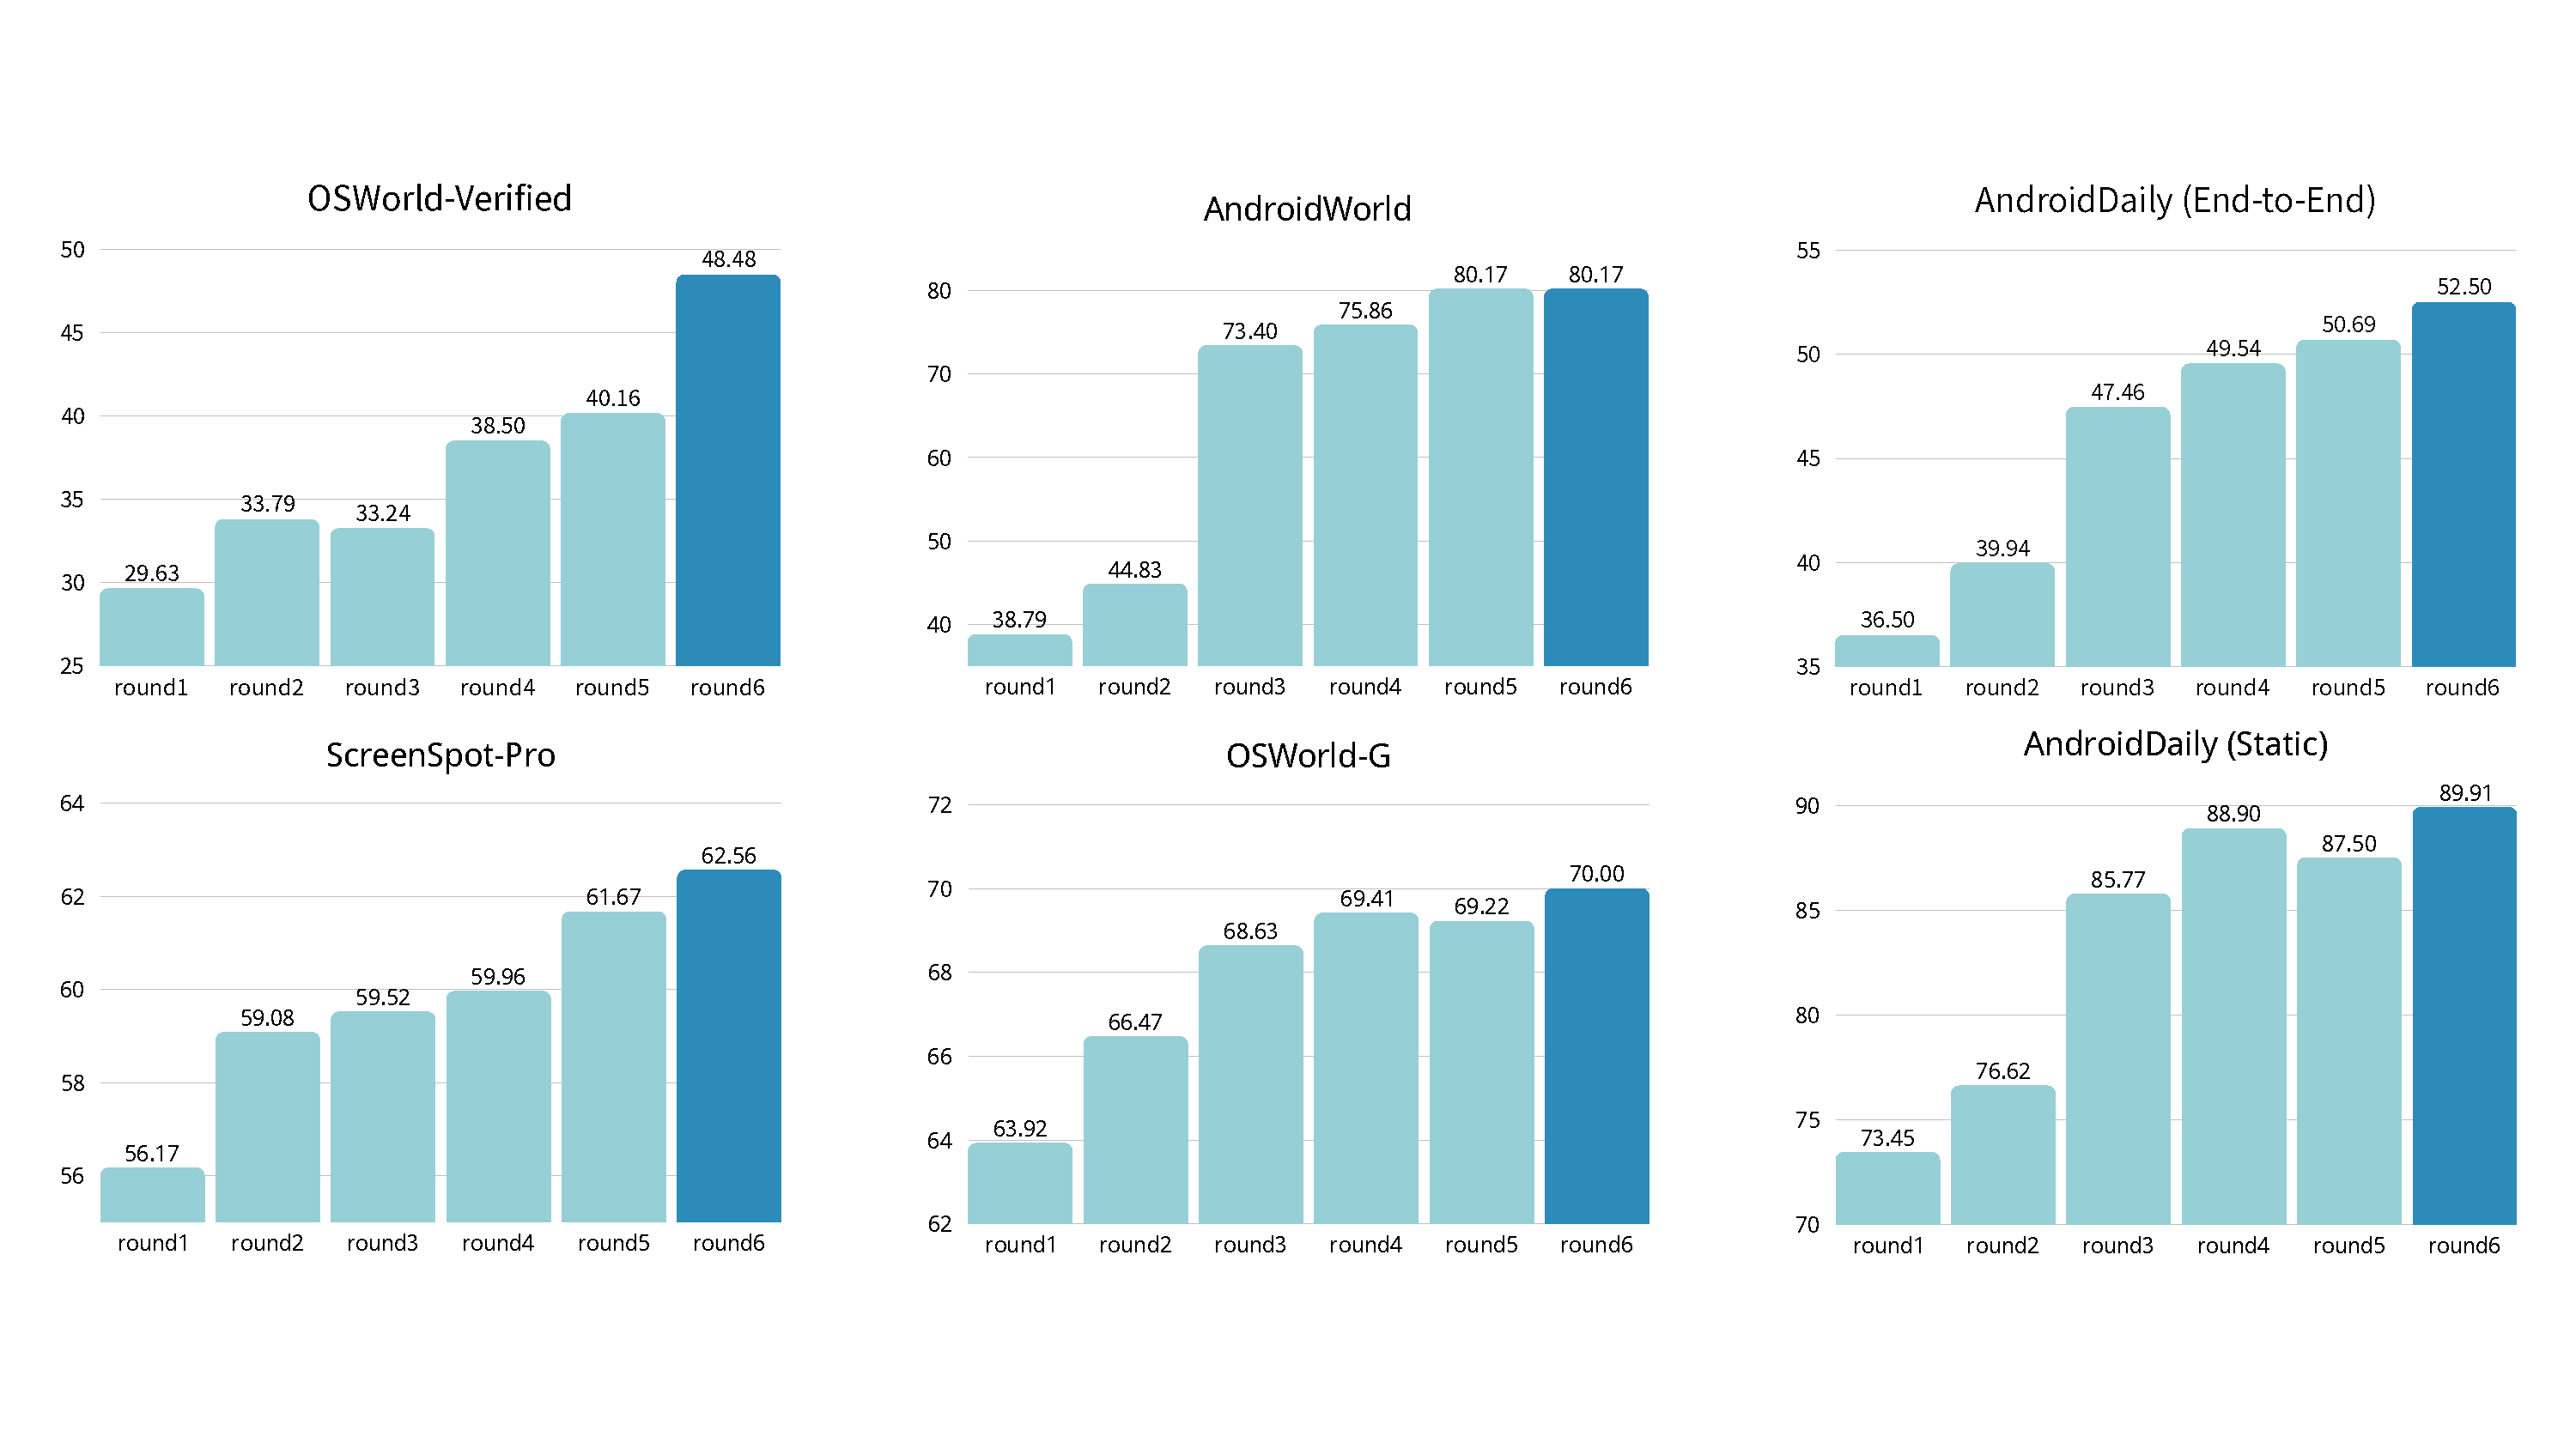
\includegraphics[width=\linewidth]{figs/self-evolving.pdf}
\caption{Step-GUI-8B 在六轮自进化训练中的性能演化。}
\label{fig:self_evolving}
\end{figure}

\paragraph{RLVR 训练稳定性。}
从奖励曲线、KL 变化、困惑度比例以及重要性采样方差等指标来看，训练过程保持了相对平稳的上升趋势，没有出现明显的奖励欺骗或发散。尤其是联合奖励和各子能力奖励的同步上升，说明模型的改进并不是偶然投机，而是来自 GUI grounding、桌面操作和手机操作等多项能力的共同提升。

\begin{figure}[t]
\centering
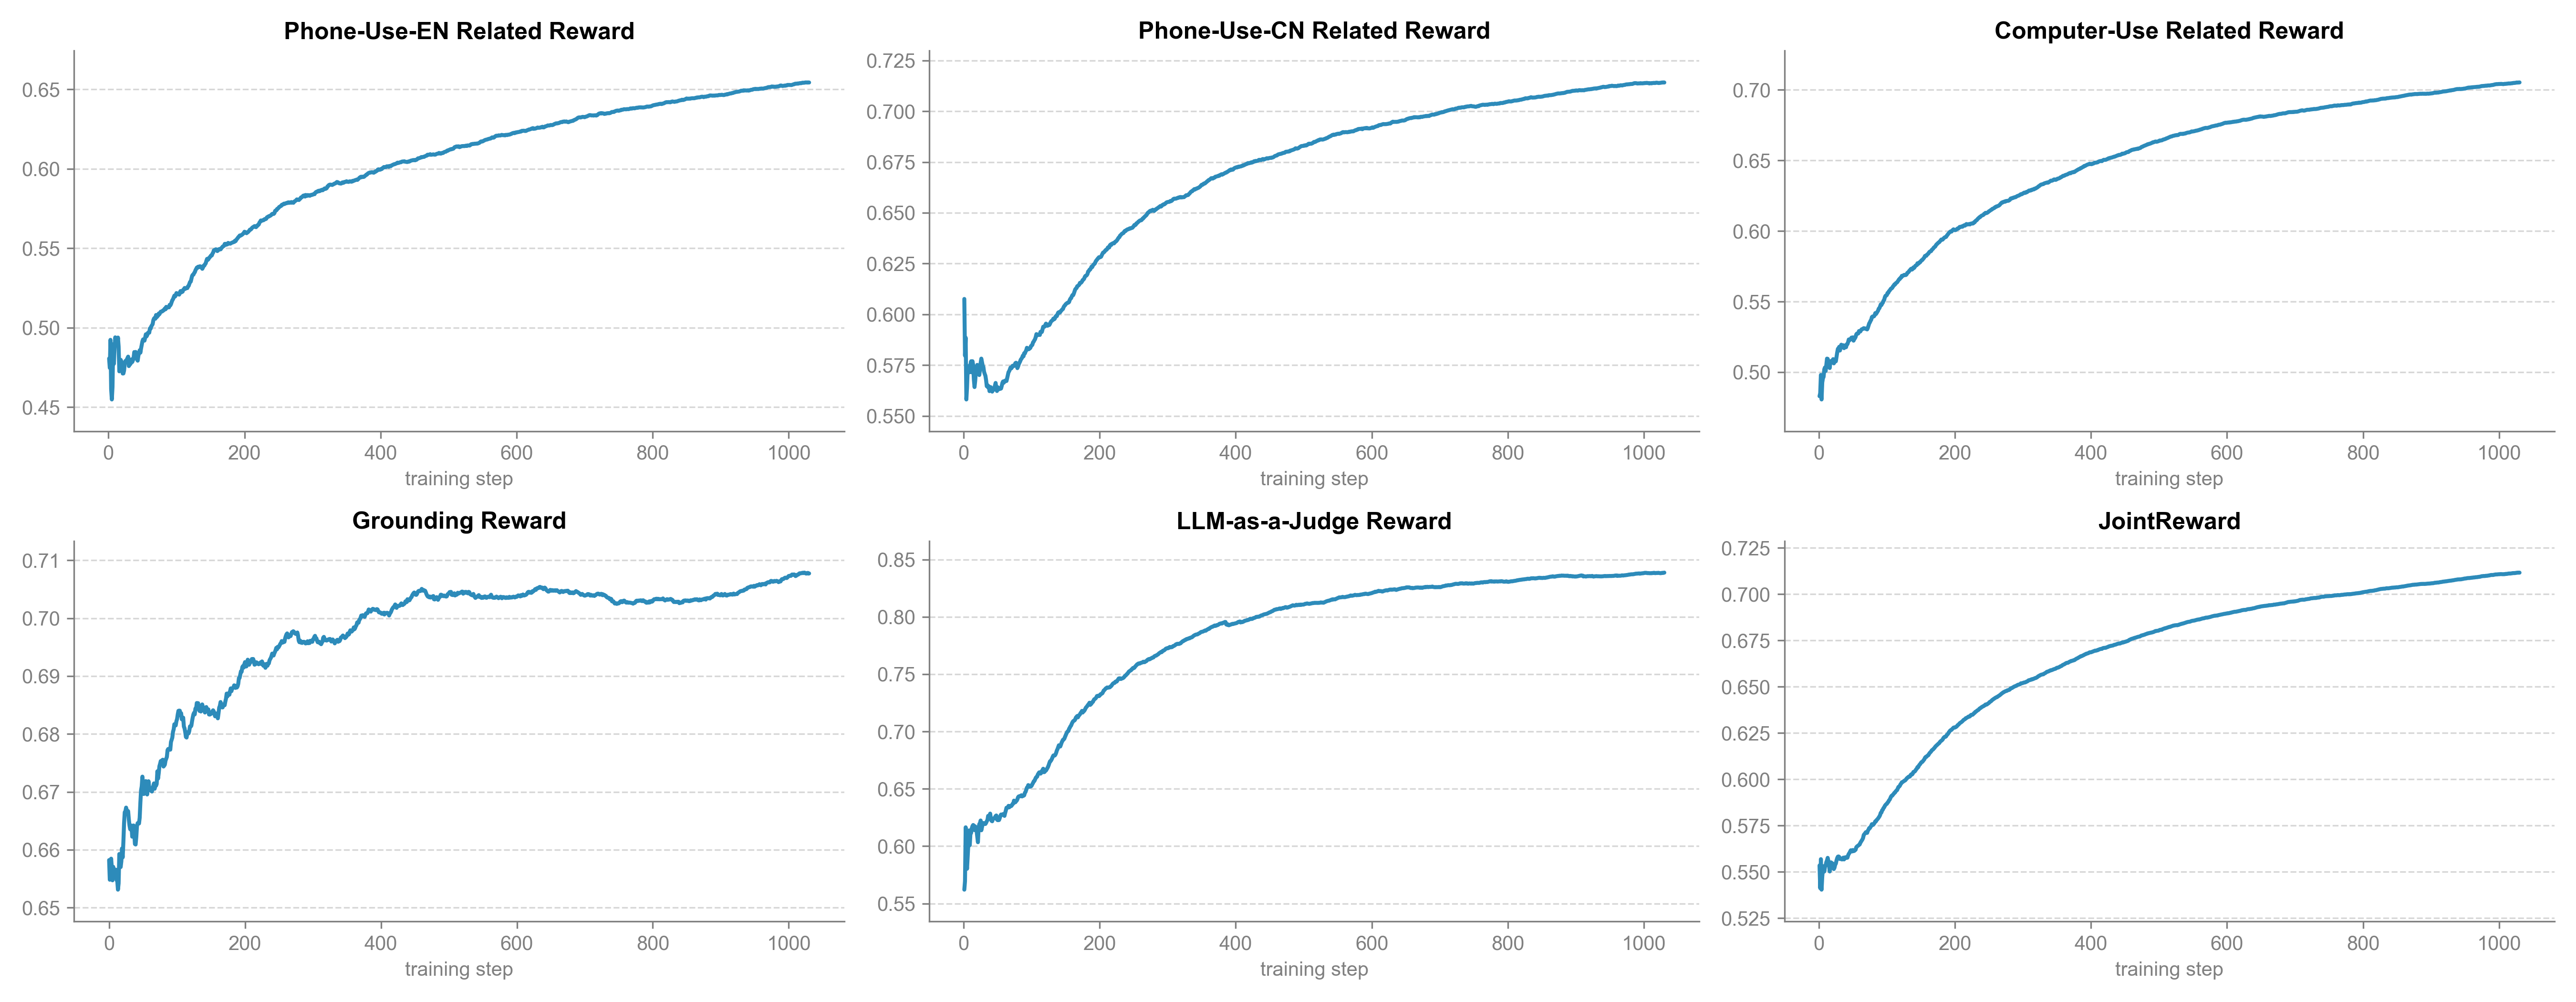
\includegraphics[width=\linewidth]{figs/training_metrics_fixed_rewards.png}
\caption{RLVR 训练过程中的奖励动态。整体曲线平滑上升，说明训练收敛稳定。}
\label{fig:joint_reward}
\end{figure}

\begin{figure}[t]
\centering
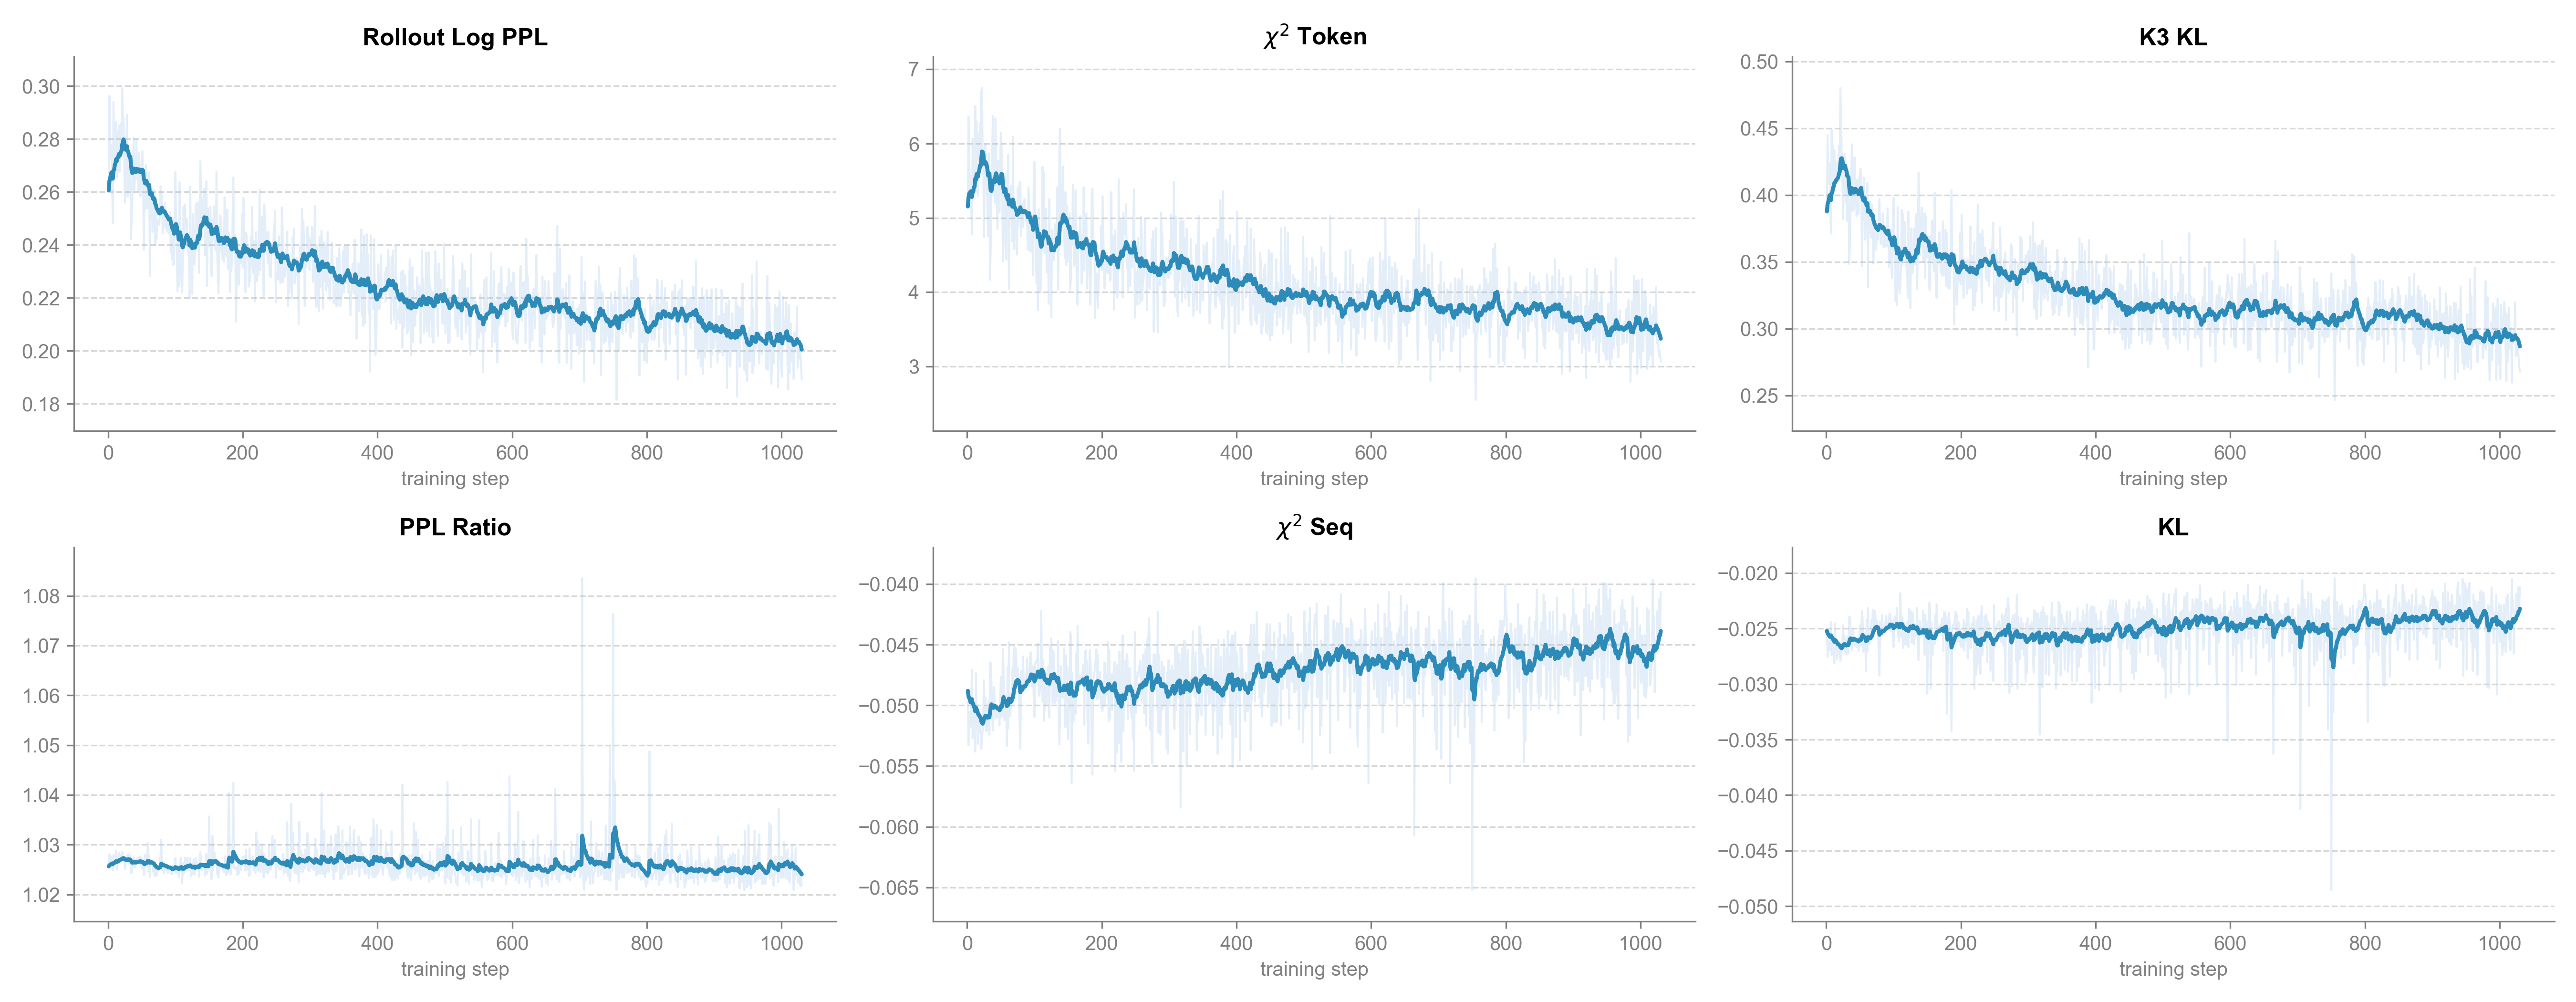
\includegraphics[width=\linewidth]{figs/training_metrics_fixed_others.png}
\caption{离策略修正与稳定性诊断结果。多项指标显示训练策略与 rollout 策略保持较高同步。}
\label{fig:joint_others}
\end{figure}

\paragraph{探索与熵。}
基础 GRPO 训练会让策略熵快速下降，虽然有助于 exploitation，但也会提高模式坍缩风险。引入梯度保持机制后，这种趋势更明显；而 Semi-Online 策略通过对失败轨迹注入少量真实提示，有效恢复了策略熵，帮助模型维持更健康的探索水平。

\begin{figure}[t]
\centering
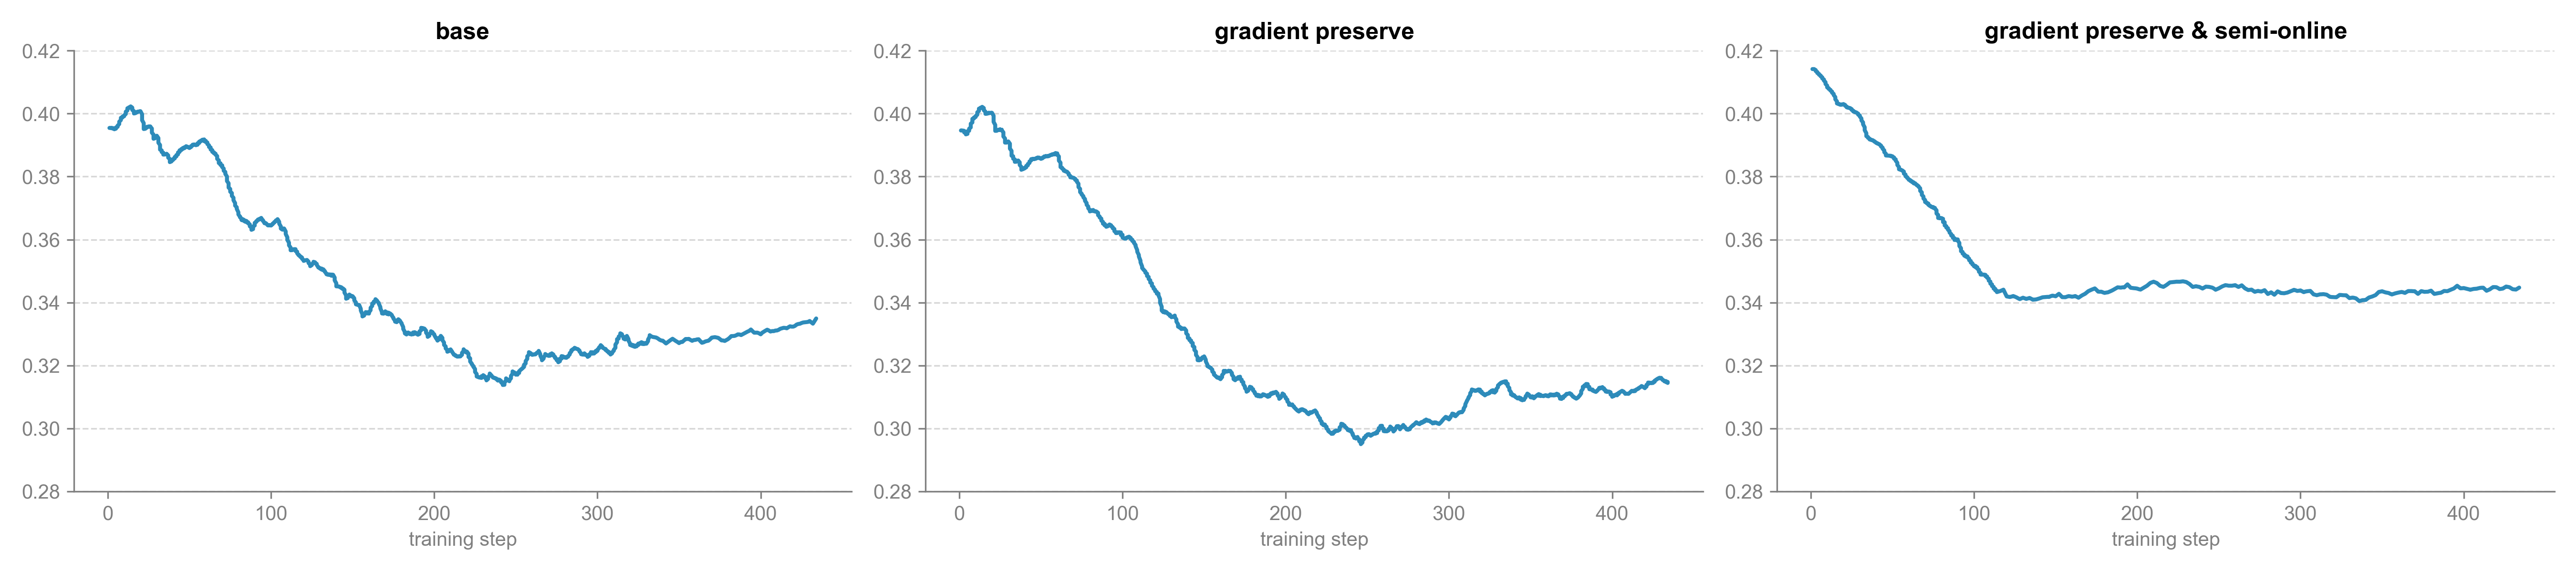
\includegraphics[width=\linewidth]{figs/training_metrics_fixed_pgz.png}
\caption{不同训练策略下策略熵的演化。Semi-Online 策略显著改善了探索水平。}
\label{fig:entropy}
\end{figure}
